\documentclass{article}

\usepackage{tikz}

\usetikzlibrary{automata,
    positioning,
    arrows,
    calc}

\begin{document}
\begin{center}
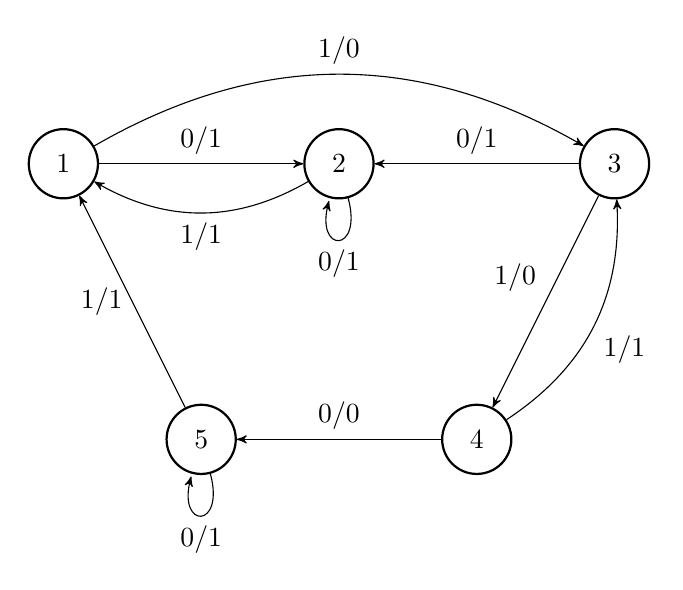
\begin{tikzpicture} [->,
    > = stealth',
    node distance = 3.5cm,
    every state/.style = {thick, fill = gray!0}]
\node[state] (q1) {$1$};  
\node[state, right of=q1] (q2) {$2$};  
\node[state, right of=q2] (q3) {$3$};  
\coordinate (midq2q3) at ($(q2)!0.5!(q3)$);
\node[state, below of=midq2q3] (q4) {$4$};  
\node[state, left of=q4] (q5) {$5$};

\draw (q1) edge[bend left, above] node{1/0} (q3);
\draw (q1) edge[above] node{0/1} (q2);

\draw (q2) edge[bend left, below] node{1/1} (q1);
\draw (q2) edge[loop below] node{0/1} (q2);

\draw (q3) edge[above] node{0/1} (q2);
\draw (q3) edge[above left] node{1/0} (q4);
    
\draw (q4) edge[above] node{0/0} (q5);
\draw (q4) edge[bend right, below right] node{1/1} (q3);

\draw (q5) edge[loop below] node{0/1} (q5);
\draw (q5) edge[left] node{1/1} (q1);
\end{tikzpicture}
\end{center}


\begin{center}
    \begin{tikzpicture}[scale = 1.75,
      transform shape, 
      thick,
      arrows = ->,
      > = Latex,
      state/.style = {circle, draw, minimum size = 30},
      accepted_state/.style = {circle, draw, double distance = 2, minimum size = 30},
      label/.style = {scale = 0.75}]
      \node[state]           (2)      {$2$};
      \node[accepted_state]  (1_2)    [below=of 2]          {$1,2$};
      \node[state]           (4)      [right=of 2]          {$4$};
      \node[accepted_state]  (3)      [below=of 4]          {$3$};
      \node[state]           (2_4)    [right=of 4]          {$2,4$};
      \node[accepted_state]  (2_3)    [below=of 2_4]        {$2,3$};
      \coordinate (vcenter)           at ($(2_4)!0.5!(2_3)$);
      \node[accepted_state]  (1_2_3)  [right=of vcenter]    {\scriptsize$1,2,3$};
      \draw ($(1_2) + (-1.5,0)$) -- (1_2);
      \draw (1_2) -- node[label, left]  {$a$} (2);
      \draw (1_2) -- node[label, above] {$b$} (3);
      %\draw (2) .. controls ($(2) + (-1,1)$) and ($(2) + (-1.5,0)$) .. (2) node[label, midway, left] {$a$};
      \draw (2) edge[-{Latex}, loop left, above] node[label, left] {$a$} (2);
      \draw (2) -- node[label, very near start, below] {$b$} (3);
      \draw (4) -- node[label, near start, above, sloped] {$a,b$} (1_2);
      \draw (3) -- node[label, right, near start] {$a$} (4);
      \draw (3) -- node[label, above] {$b$} (2_3);
      \draw (2_4) -- node[label, very near start, above] {$a$} (1_2);
      \draw (2_4) -- node[label, above] {$b$} (1_2_3);
    \end{tikzpicture}
  \end{center}

  \begin{center}
    \begin{tikzpicture}[scale = 1.75, transform shape, thick, -{Latex}]
      \node[circle, draw, double distance = 2]  (q_1)                   {$q_1$};
      \node[circle, draw, double distance = 2]  (q_2)   [right=of q_1]  {$q_2$};
      \node[circle, draw, double distance = 2]  (q_3)   [right=of q_2]  {$q_3$};
      \node[circle, draw, double distance = 2]  (q_4)   [right=of q_3]  {$q_4$};
      \node[circle, draw]                       (q_5)   [right=of q_4]  {$q_5$};
      \draw (-1,0) -- (q_1);
      \draw (q_1) -- node[above, scale = 0.75] {$y$} (q_2);
      \draw (q_2) -- node[above, scale = 0.75] {$x$} (q_3);
      \draw (q_3) -- node[above, scale = 0.75] {$x$} (q_4);
      \draw (q_4) -- node[above, scale = 0.75] {$y$} (q_5);
      \draw (q_1) edge[loop above] node[above] {$x$} (q_1);
      %\draw (q_1) .. controls ($(q_1) + (.75,1)$)   and ($(q_1) + (-.75,1)$) ..   (q_1) node[midway, above, scale = 0.75]   {$x$};
      \draw (q_2) .. controls ($(q_2) + (0,1)$)     and ($(q_2) + (-1.25,1)$) ..  (q_2) node[midway, above, scale = 0.75]   {$y$};
      \draw (q_3) .. controls ($(q_3) + (-.25,1)$)  and ($(q_2) + (.25,1)$) ..    (q_2) node[midway, above, scale = 0.75]   {$y$};
      \draw (q_4) .. controls ($(q_4) + (-.25,-1)$) and ($(q_1) + (.25,-1)$) ..   (q_1) node[midway, below, scale = 0.75]   {$x$};
      \draw (q_5) .. controls ($(q_5) + (.75,1)$)   and ($(q_5) + (-.75,1)$) ..   (q_5) node[midway, above, scale = 0.75]   {$x,y$};
    \end{tikzpicture}
  \end{center}

  \end{document}